\chapter{Experiments and Data Collection}\label{chapter:expt-data-collection}
Motivation: Sleep is an essential behavioral program conserved across the animal kingdom.
In mammals sleep consists of multiple stages marked by physiological changes including reductions in muscle tone and distinct electrophysiological activity patterns in the brain.
In invertebrates, sleep has largely been studied as a unitary process and identified by bouts of consolidated immobility.
Thus, careful characterization of underlying changes in behavior and physiology is needed to characterize distinct sleep stages in powerful genetic model systems such as Drosophila.

\begin{figure}[ht!]
	\centering
	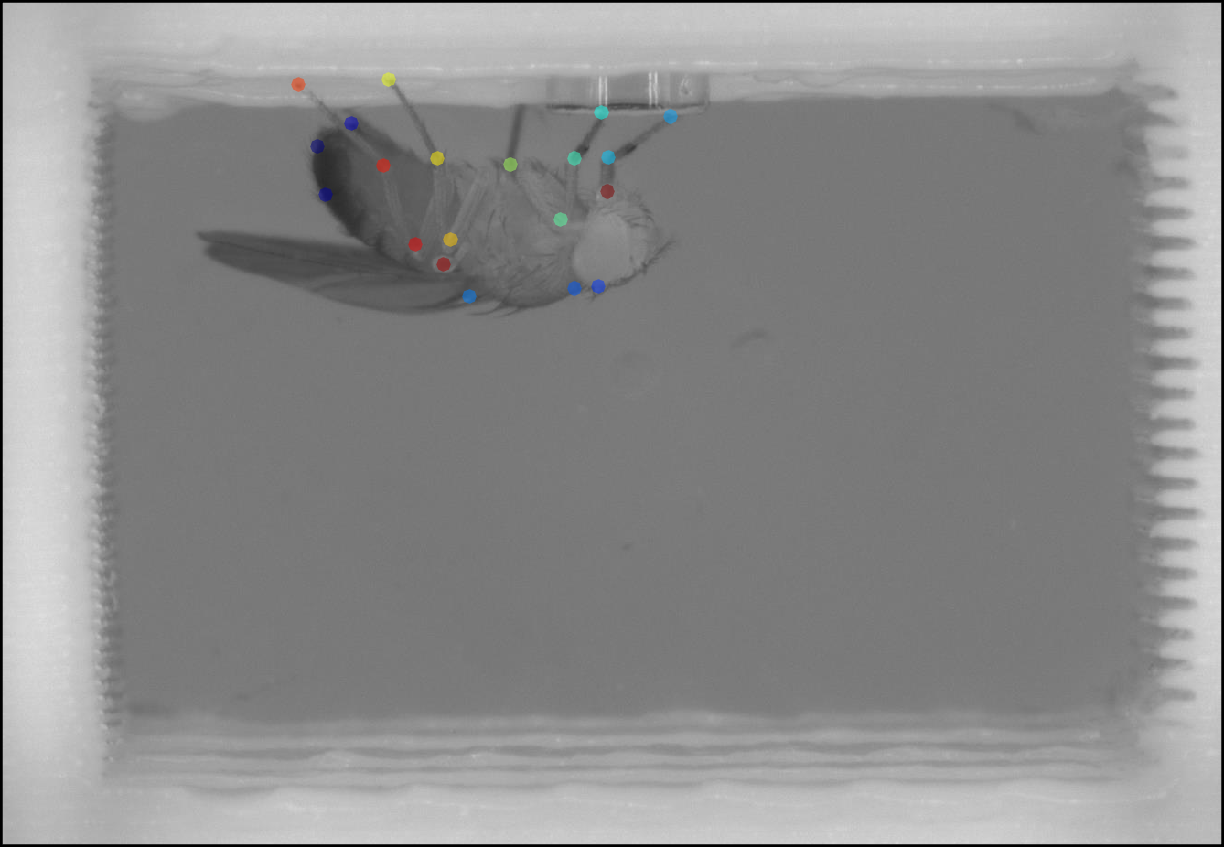
\includegraphics[width=0.75\linewidth]{figures/FlyTrackedBodyParts.png}
	\caption{}
\end{figure}

\begin{figure}[ht!]
	\centering
	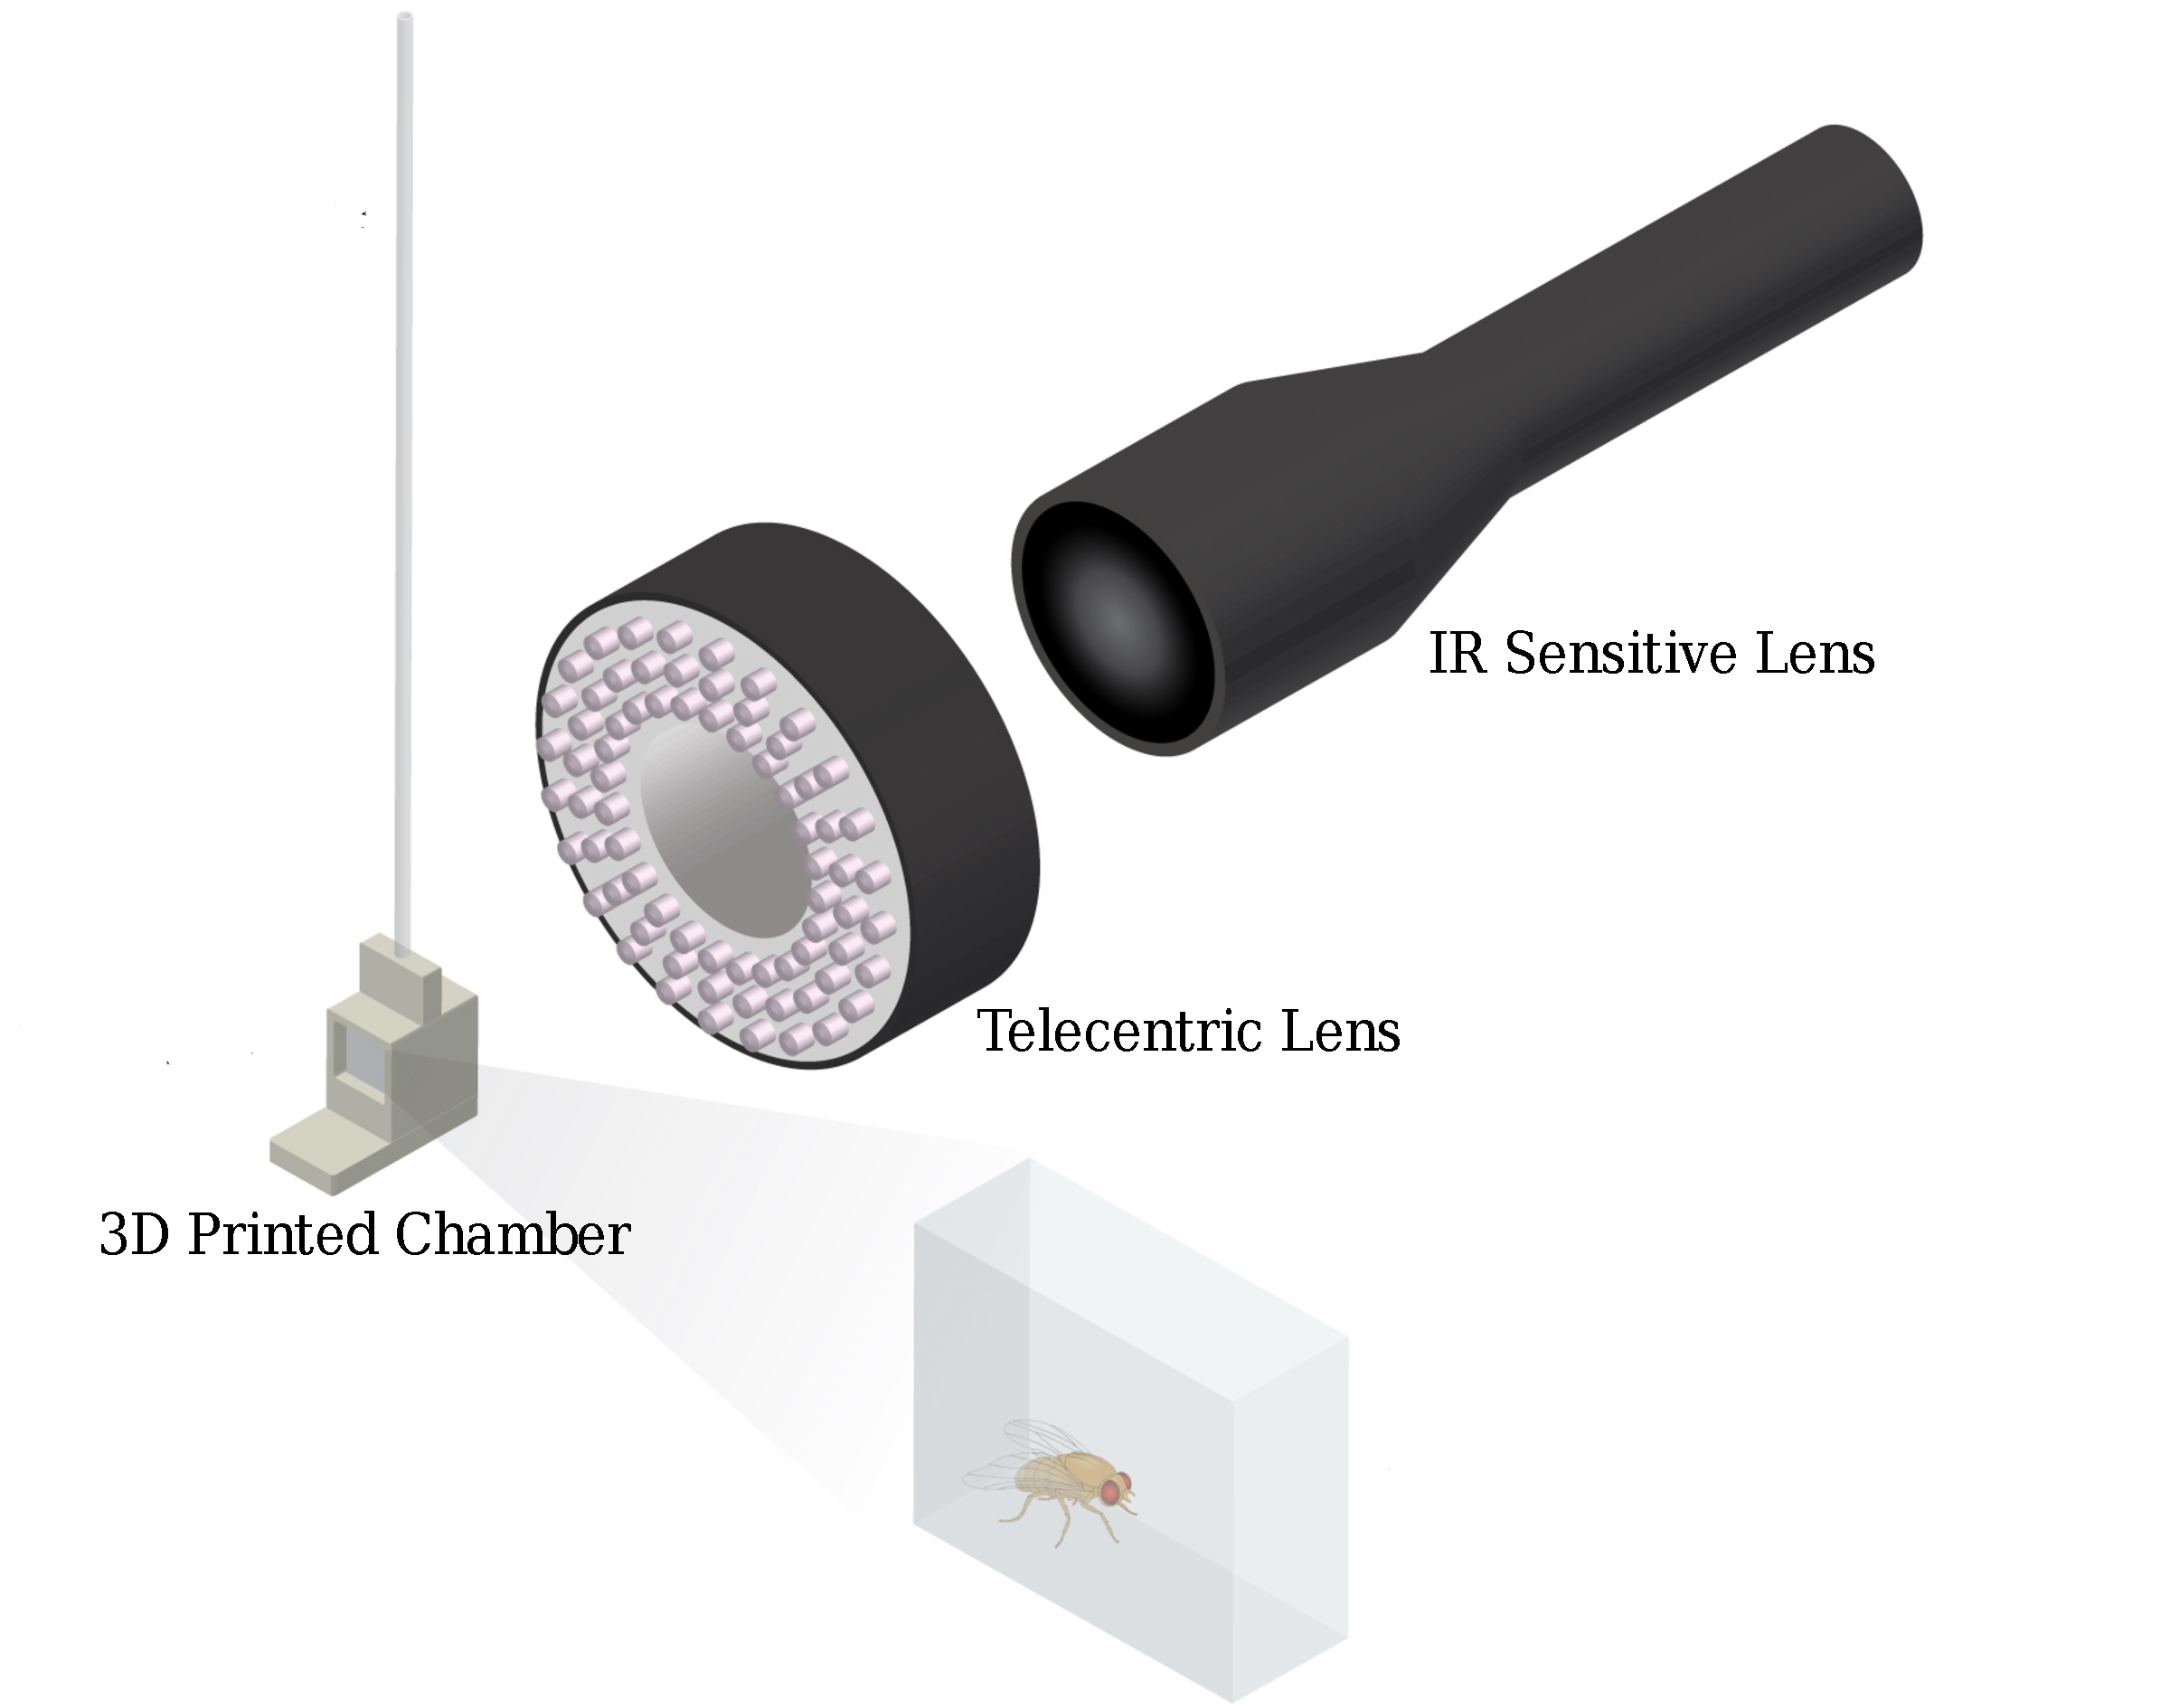
\includegraphics[width=0.75\linewidth]{figures/ExperimentalSetup.pdf}
	\caption{}
\end{figure}
Experimental Setup: We developed a custom imaging setup to perform high-resolution characterization of sleep-related behaviors in flies.
A custom 3D printed chamber (7.2X4.3X2.4 mm [WxHxL]) is placed in front of a IR sensitive (Flir) camera with telecentric lens (Edmund Optics).
Flies recorded from ZT10-ZT2 (16 hours) total.
Each chamber has a food port (1.5mm diameter) that allows access to liquid food (2.5\% yeast, 2.5\% sugar).
Recording setup is in light tight box and humidity control (60\%) is achieved via humidifier plugged into a humidity control switch.
Experimental flies are loaded to individual chambers at ZT8-ZT9 via mouth pipette or a small vacuum pump.
Individual chambers are sealed with a 7x7 mm acrylic windows.
Windows are coated with SigmaCote to prevent flies from ventral or dorsal postural positions.
5-7 day old female and male flies are used in the experiments.

\begin{figure}[ht!]
	\centering
	\begin{subfigure}[ht!]{0.95\linewidth}
		\centering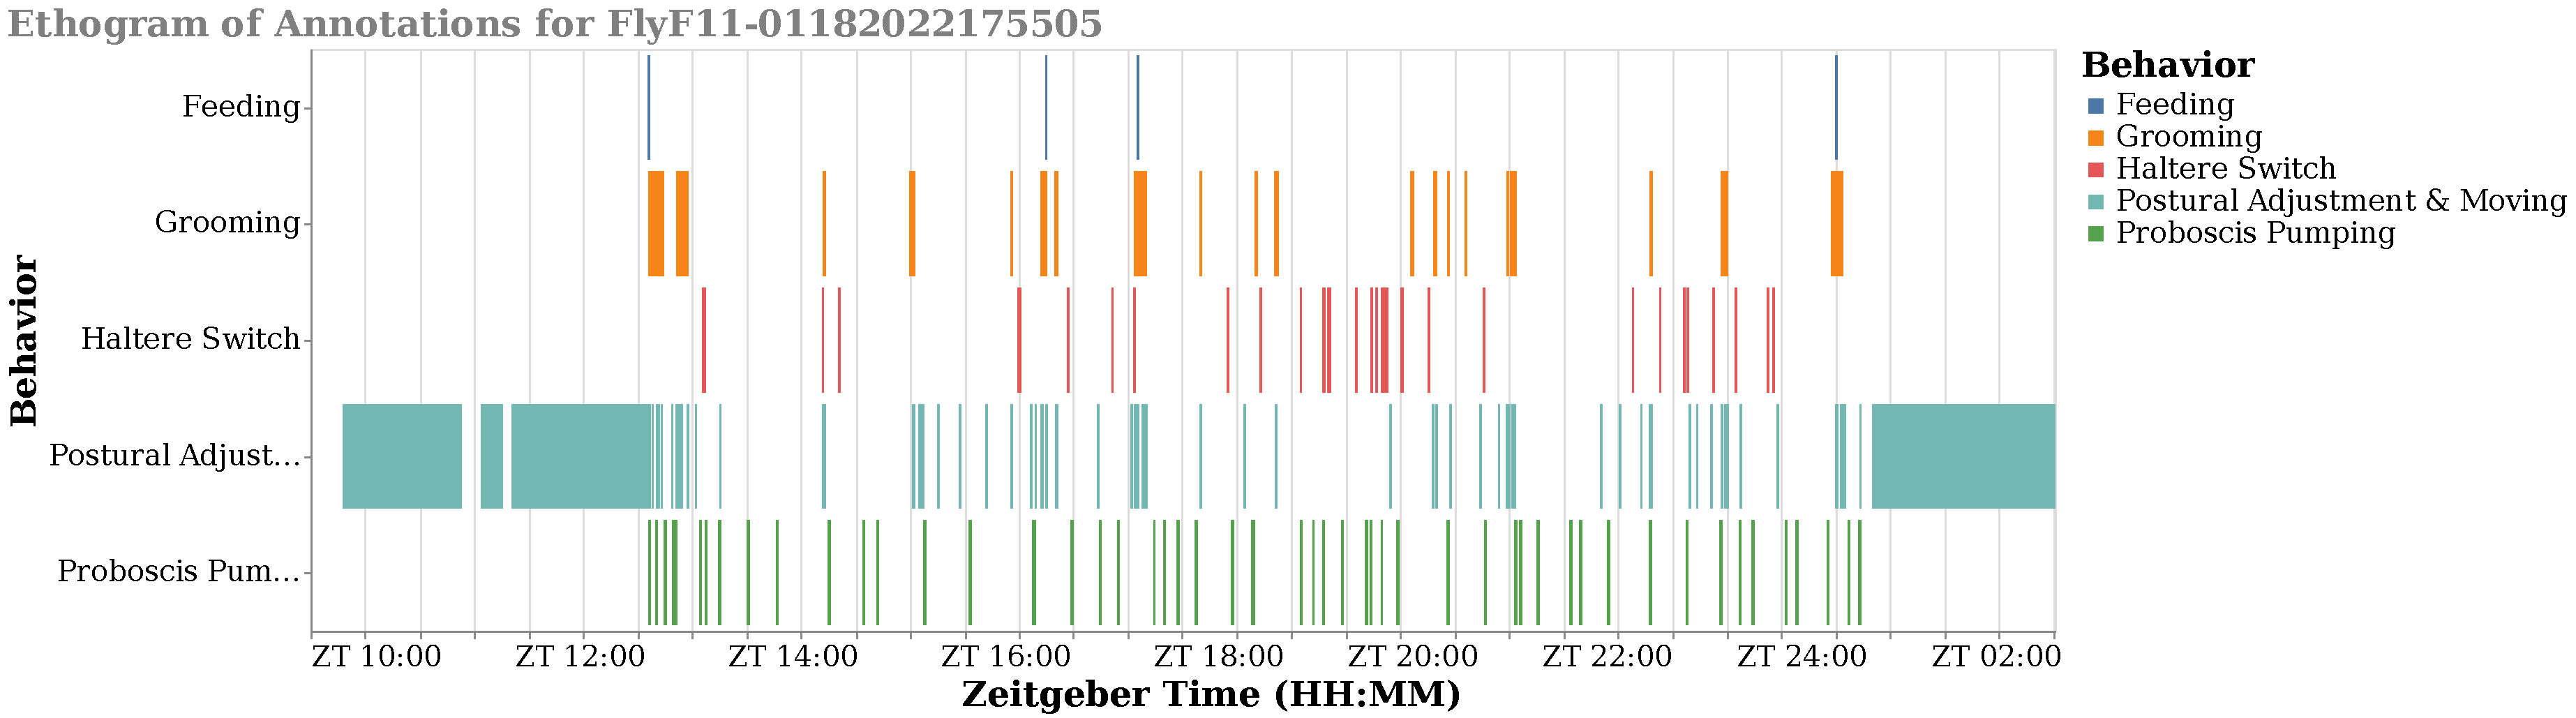
\includegraphics[width=\linewidth]{figures/FlyF11-01182022175505_annotation_ethogram.pdf}
		\caption{}
	\end{subfigure}%

	\centering
	\begin{subfigure}[ht!]{0.95\linewidth}
		\centering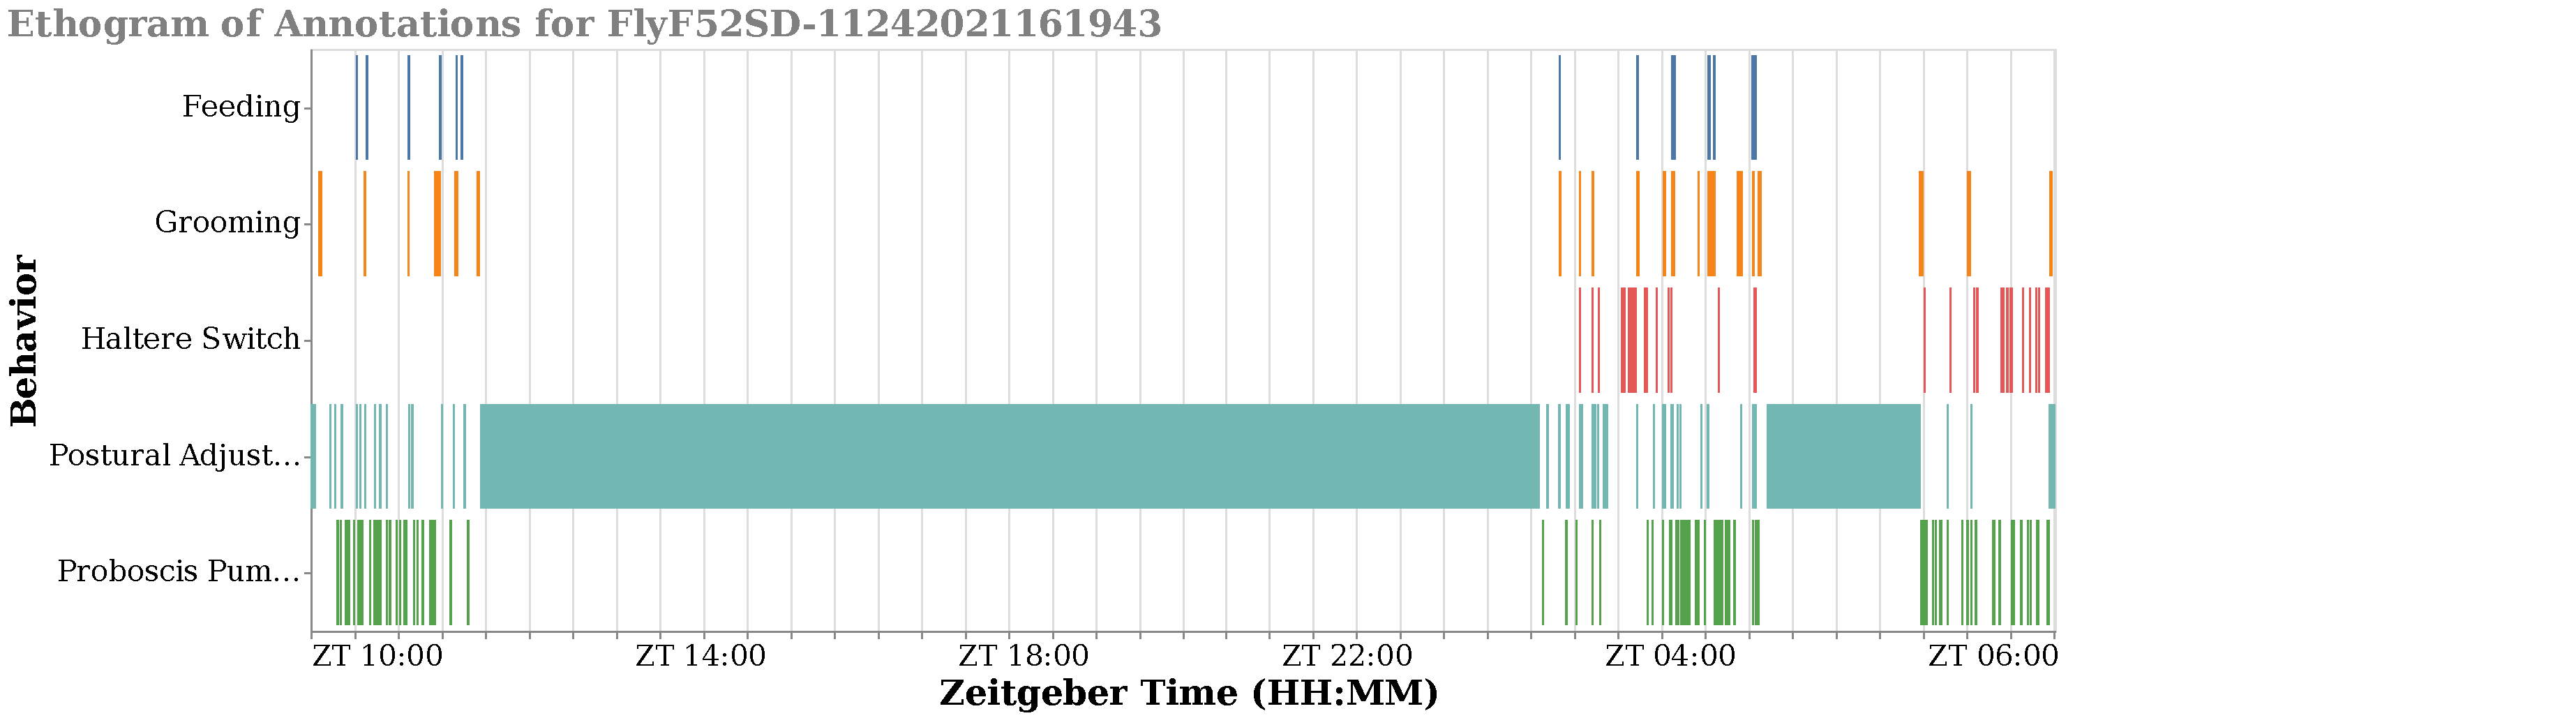
\includegraphics[width=\linewidth]{figures/FlyF52SD-11242021161943_annotation_ethogram.pdf}
		\caption{}
	\end{subfigure}%
	\caption{}
\end{figure}

Annotations: 3 annotators labeled 5 different behaviors (feeding, grooming, moving, haltere switch, proboscis pumping) across 10 videos (16 hour each).
A single experiment is annotated by all 3 annotators to check rigor and overlap among annotators.
90\% coverage is required among annotators to proceed with annotation of a novel fly.
